\documentclass[varwidth]{standalone}
\usepackage{tikz}
\usepackage{pgfplots}
\usepgfplotslibrary{fillbetween}
\begin{document}
    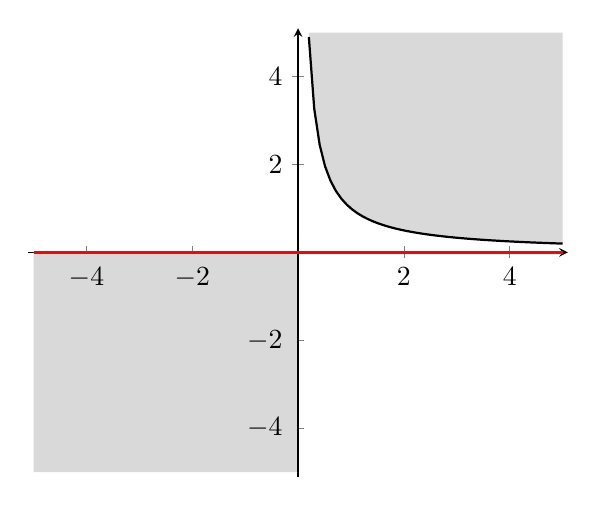
\begin{tikzpicture}
        \begin{axis}[
            axis lines = center,
            ymin=-5,
            ymax=5,
            restrict y to domain=-5:5,
            xmin=-5,
            xmax=5,
            restrict x to domain=-5:5,
            enlargelimits=0.01
        ]
            \path[name path=upperaxis] (axis cs:0.2,5) -- (axis cs:5,5);
            \path[name path=loweraxis] (axis cs:0,-5) -- (axis cs:-5,-5);
            \addplot[name path=upper, domain=0:5, samples=50, thick] {1 / x};
            \addplot[fill=gray!30] fill between [of=upperaxis and upper];
            \addplot[name path=lower, domain=-5:0, samples=50, thick] {0};
            \addplot[fill=gray!30] fill between [of=loweraxis and lower];
            \addplot[thick] coordinates {(0, 0) (0, -5)};
            \addplot[very thick, domain=-5:5, color=red] {0};
        \end{axis}
    \end{tikzpicture}
\end{document}